% !TeX root = surprises.tex

\chapter{Solving Quadratic Equations}\label{c.quadratic}

%%%%%%%%%%%%%%%%%%%%%%%%%%%%%%%%%%%%%%%%%%%%%%%%%%%%%%%%%%%%%%%

Poh-Shen Loh\index{Loh, Poh-Shen} schlug eine Methode zum Lösen quadratischer Gleichungen vor, die auf einer Beziehung zwischen den Koeffizienten des quadratischen Polynoms und seinen Wurzeln beruht. Abschnitt~\ref{s.traditional} gibt einen Überblick über die traditionellen Methoden zum Lösen quadratischer Gleichungen. 
Abschnitt~\ref{s.computing} versucht, den Leser davon zu überzeugen, dass die Loh-Methode sinnvoll ist, und erklärt dann, wie man die Wurzeln berechnet. In Abschnitt~\ref{s.examples} wird die Berechnung für zwei quadratische Polynome und eine ähnliche Berechnung für ein quartisches Polynom durchgeführt. In Abschnitt~\ref{s.general} wird die traditionelle Formel für die Wurzeln aus den Loh'schen Formeln abgeleitet.

Die Einführung der Algebra und der modernen algebraischen Notation ist relativ neu. Zuvor benutzten die Mathematiker fast ausschließlich die Geometrie, so dass es interessant ist, al-Khwarizmis geometrische Konstruktion der Formel für die Wurzeln quadratischer Gleichungen zu betrachten (Sect.~\ref{s.khwar}). Abschnitt~\ref{s.cardano} zeigt eine geschickte geometrische Konstruktion, die Cardano bei der Entwicklung der Formel für die Wurzeln kubischer Gleichungen verwendet hat.

Abschnitt~\ref{s.lill-quadratic} stellt andere geometrische Methoden zum Auffinden der Wurzeln quadratischer Gleichungen vor.\footnote{Kapitel~\ref{c.origami-cube} ist eine Voraussetzung für das vollständige Verständnis dieser Methoden.} Das Kapitel schließt mit dem Abschnitt ~\ref{s.numerical} ab, der die numerische Berechnung der Wurzeln quadratischer Gleichungen behandelt.

\section{Traditionelle Methoden zum Lösen quadratischer Gleichungen}\label{s.traditional}
\index{Quadratische Gleichung}
Jeder Mathematikstudent kennt die Formel für die Ermittlung der Wurzeln einer quadratischen Gleichung $ax^2+bx+c=0$ auswendig:
\[
x_1, x_2 = \frac{-b\pm\sqrt{b^2-4ac}}{2a}\,.
\]                      
Für den Moment arbeiten wir mit monischen Polynomen, $x^2+bx+c=0$, deren Wurzeln sind:
\begin{align}
x_1, x_2 = \frac{-b\pm\sqrt{b^2-4c}}{2}\,.\label{eq.quadratic-roots}
\end{align}
Eine andere Methode, quadratische Gleichungen zu lösen, besteht darin, die Polynome mehr oder weniger durch Versuch und Irrtum zu faktorisieren. Manchmal ist es einfach, die Wurzeln durch Faktorisierung zu erhalten:
\begin{align}
x^2-4x+3= (x-1)(x-3)\label{eq.quadratic-lill}\,.
\end{align}
Es ist viel schwieriger, $x^2-2x-24$ zu faktorisieren, weil es viele mögliche Wurzelpaare gibt, die berücksichtigt werden müssen:
\[
(\pm 1,\mp 24)\,, (\pm 2,\mp 12)\,, (\pm 3,\mp 8)\,, (\pm 4,\mp 6)\,.
\]

\section{Die Beziehung zwischen den Wurzeln und den Koeffizienten}\label{s.computing}
\index{Quadratic equation!roots of}
\begin{theorem}\label{thm.roots-coefficients}
Wenn $r_1,r_2$ die Wurzeln von $x^2+bx+c$ sind, dann:
\[
(x-r_1)(x-r_2)=x^2 - (r_1+r_2)x + r_1r_2=x^2+bx+c\,.
\]
Auch wenn wir die Werte der Wurzeln nicht kennen, so wissen wir doch, dass:
\begin{align}\label{eq.viete-quad}
r_1+r_2 = -b\,,\quad\quad r_1r_2=c\,.
\end{align}
\end{theorem}

Es gibt eigentlich nichts zu beweisen, denn das Ergebnis ergibt sich aus der Berechnung.

Betrachte einige Werte von $-b,r_1,r_2$ und sei $m_{12}$ der Durchschnitt von $r_1,r_2$:
\[
\renewcommand{\arraystretch}{1.2}
\begin{array}{|@{\hspace{1em}}r|@{\hspace{1em}}r|@{\hspace{1em}}r|@{\hspace{1em}}r|}
\hline
-b& r_1 & r_2 &m_{12}\\\hline
33 & 12 & 21 & 16\frac{1}{2}\\\hline
33 & 8 & 25 & 16\frac{1}{2}\\\hline
33 & 1 & 32 & 16\frac{1}{2}\\\hline\hline
-b& r_1 & r_2 &m_{12}\\\hline
-4 & -16 & 12 & -2 \\\hline
-4 & -4 & 0 & -2 \\\hline
-4 & -3 & -1 & -2 \\\hline
\end{array}
\]
Bei jeder quadratischen Gleichung ist der Durchschnitt der beiden Wurzeln konstant:
\[
m_{1,2}=\frac{r_1+r_2}{2}=
\frac{(-b-r_2)+r_2}{2}=
-\frac{b}{2}\,.
\]
Sei $s$ eine beliebige Zahl. Dann:
\[
-b=-b+s+(-s)=\left(\frac{-b}{2}+s\right) + \left(\frac{-b}{2}-s\right)=r_1+r_2\,.
\]
Wenn eine Wurzel im Abstand $s$ vom Durchschnitt liegt, liegt die andere Wurzel im Abstand $-s$ vom Durchschnitt. Für $r_1,r_2=2,6$, mit $m_{12}=4, s=2$, haben wir:
\[
\renewcommand{\arraystretch}{1.2}
\begin{array}{|@{\hspace{1em}}r|@{\hspace{1em}}r|@{\hspace{1em}}r|@{\hspace{1em}}r|r|r|}
\hline
-b& r_1 & r_2 & m_{12}& m_{12}\!-\!r_1 & m_{12}\!-\!r_2\\\hline
33 & 12 & 21 & 16\frac{1}{2}&4\frac{1}{2} & -4\frac{1}{2}  \\\hline
33 & 8 & 25 & 16\frac{1}{2}&8\frac{1}{2}&-8\frac{1}{2}\\\hline
33 & 1 & 32 & 16\frac{1}{2}&15\frac{1}{2}&-15\frac{1}{2}\\\hline
\hline
-4 & -16 & 12 & -2 &14& -14\\\hline
-4 & -4 & 0 & -2&2&-2 \\\hline
-4 & -3 & -1 & -2&1&-1 \\\hline
\end{array}
\]
Abbildung~\ref{f.loh-roots1} veranschaulicht diese Beziehung.
\begin{figure}[t]
\begin{center}
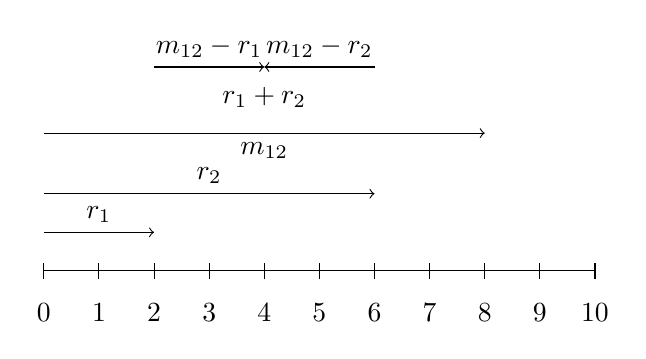
\begin{tikzpicture}[scale=.7]
\begin{scope}[yshift=-4mm]
\draw (0,0) -- (10,0);
\foreach \x in {0,1,...,10}
  \draw (\x,-1.5mm) -- +(0,3mm) node[below,yshift=-4mm] {$\x$};
\draw[->,yshift=7mm] (0,0) -- node[above] {$r_1$} (20mm,0);
\draw[->,yshift=14mm] (0,0) -- node[above] {$r_2$} (60mm,0);
\end{scope}
\draw[->,yshift=21mm] (0,0) -- node[above,yshift=2mm] {$r_1+r_2$} (80mm,0);
\coordinate (M) at (40mm,21mm);
\vertex{M};
\node[below] at (40mm,21mm) {$m_{12}$};
\begin{scope}[yshift=3mm]
\draw[->,yshift=30mm] (20mm,0mm) -- node[above] {$m_{12}-r_1$} +(20mm,0);
\draw[->,yshift=30mm] (60mm,0mm) -- node[above] {$m_{12}-r_2$} +(-20mm,0);
\end{scope}
\end{tikzpicture}
\end{center}
\caption{Beziehung zwischen den Wurzeln $r_1,r_2=2,6$ und ihrem Durchschnitt $m_{12}=4$}
\label{f.loh-roots1}
\end{figure}
If we use other values $r_1,r_2=3,5$ for which $r_1+r_2=8$ then $m_{12}=4$ bleibt gleich, während $s$ zu $1$ wird (Abb.~\ref{f.loh-roots2}).

Der Versatz $s$ scheint in willkürlich zu sein:
\[
r_1=\left(\frac{-b}{2}+s\right)\,,\quad r_2=\left(\frac{-b}{2}-s\right)\,,
\]
\noindent{}aber es gibt eine zusätzliche Bedingung $r_1r_2=c$, wobei $c$ der konstante Term des Polynoms ist.
Durch Multiplikation der beiden Ausdrücke, die wir für $r_1,r_2$ abgeleitet haben, können wir $s$ und dann $r_1,r_2$ bestimmen:
\begin{eqnarray*}
c&=&\left(-\frac{b}{2} +s\right)\left(-\frac{b}{2} -s\right)=
  \frac{b^2}{4}-s^s\\
s&=&\frac{\sqrt{b^2-4c}}{2}\,.
\end{eqnarray*}

\begin{figure}[t]
\begin{center}
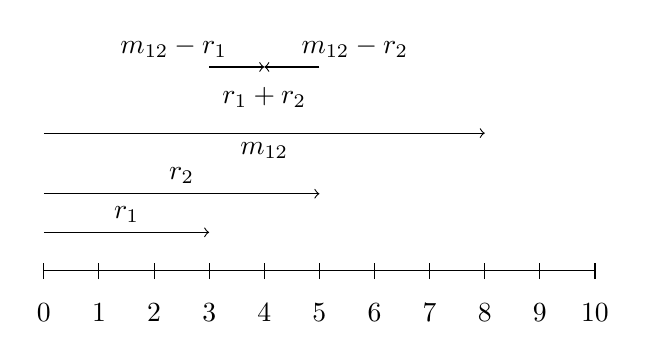
\begin{tikzpicture}[scale=.7]
\begin{scope}[yshift=-4mm]
\draw (0,0) -- (10,0);
\foreach \x in {0,1,...,10}
  \draw (\x,-1.5mm) -- +(0,3mm) node[below,yshift=-4mm] {$\x$};
\draw[->,yshift=7mm] (0,0) -- node[above] {$r_1$} (30mm,0);
\draw[->,yshift=14mm] (0,0) -- node[above] {$r_2$} (50mm,0);
\end{scope}
\draw[->,yshift=21mm] (0,0) -- node[above,yshift=2mm] {$r_1+r_2$}(80mm,0);
\coordinate (M) at (40mm,21mm);
\vertex{M};
\node[below] at (40mm,21mm) {$m_{12}$};
\begin{scope}[yshift=3mm]
\draw[->,yshift=30mm] (30mm,0mm) -- node[above left] {$m_{12}-r_1$} +(10mm,0);
\draw[->,yshift=30mm] (50mm,0mm) -- node[above right] {$m_{12}-r_2$} +(-10mm,0);
\end{scope}
\end{tikzpicture}
\end{center}
\caption{Relation between the roots $r_1,r_2=3,5$ and their average $m_{12}=4$}
\label{f.loh-roots2}
\end{figure}

\section{Examples of Loh's Method}\label{s.examples}

\begin{example}
Betrachten Sie das Polynom $x^2-2x-24$ mit $b=-2,c=-24$:
\begin{eqnarray*}
c&=&\left(-\frac{(-2)}{2} +s\right)\left(-\frac{(-2)}{2} -s\right)\\
-24&=&(1 +s)(1 -s)\\
%s^2&=&25\\
s&=&5\\
r_1&=&1+5=6\\
r_2&=&1-5=-4\,.
\end{eqnarray*}
Siehe: $(x-6)(x-(-4))= x^2-2x-24$.
\end{example}

\begin{example}
Finden wir die Wurzeln von $x^2-83x-2310$:
\begin{eqnarray*}
%c&=&\left(-\frac{b}{2} +s\right)\left(-\frac{b}{2} -s\right)\\
-2310&=&\left(\frac{83}{2}+s\right)\left(\frac{83}{2} -s\right)\\
s^2&=&\frac{6889}{4}+2310=\frac{16129}{4}\\
s&=&\frac{127}{2}\\
r_1&=&\frac{83}{2}-\frac{127}{2}=-22\\
r_2&=&\frac{83}{2}+\frac{127}{2}=105\,.
\end{eqnarray*}
Siehe: $(x+22)(x-105)= x^2-83x-2310$.

Vergleichen Sie diese Berechnung mit der Berechnung nach der traditionellen Formel:
\begin{eqnarray*}
\frac{-b\pm\sqrt{b^2-4c}}{2}&=&\frac{-(-83)\pm\sqrt{(-83)^2-4\cdot (-2310)}}{2}\\
%&=& \frac{83\pm\sqrt{6889+9240}}{2} = \frac{83\pm\sqrt{16129}}{2}\\
&=& \frac{83\pm\sqrt{16129}}{2} = \frac{83\pm 127}{2}\\
r_1&=&\frac{83-127}{2}=-22\\
r_2&=&\frac{83+127}{2}=105\,.
\end{eqnarray*}
\end{example}

\begin{example}
Theorem~\ref{thm.roots-coefficients} kann auf Polynome höheren Grades verallgemeinert werden. Hier ist ein interessantes Beispiel für eine \emph{quartische Gleichung}\index{Quartische Gleichung} $x^4-10x^2-x+20=0$. Wie für quadratische Gleichungen gibt es auch für kubische und quartische Gleichungen (allerdings nicht für Gleichungen höherer Potenzen) Formeln zum Lösen, aber die Formeln sind recht kompliziert.

Kann dieses Polynom vierten Grades in zwei quadratische Polynome mit ganzzahligen Koeffizienten zerlegt werden? Wenn ja, müssen die Koeffizienten der $x$-Terme \emph{gleich und mit entgegengesetztem Vorzeichen} sein, da der Koeffizient des $x^3$-Terms Null ist. Daher lautet die Form der quadratischen Faktoren:
\[
f(x) = (x^2 - nx + k_1)\, (x^2 + nx + k_2)\,.
\]
Die Durchführung der Multiplikation ergibt:
\[
\renewcommand{\arraystretch}{1.1}
\begin{array}{rrrrrr}
f(x) = &x^4 & + nx^3 & + k_2 x^2\\
&& -nx^3 &- n^2x^2 &-nk_2x\\
&&&+k_1x^2 &+ nk_1x &+ k_1k_2\,.
\end{array}
\]
Die Gleichsetzung der Koeffizienten ergibt drei Gleichungen in den drei Unbekannten $n,k_1,k_2$ ergibt:
\begin{eqnarray*}
(k_1+k_2)-n^2 &=& -10\\
n(k_1-k_2) &=& -1\\
k_1k_2 &=& 20\,.
\end{eqnarray*}
Da wir nach Faktoren mit ganzzahligen Koeffizienten suchen, ergibt sich aus den letzten beiden Gleichungen, dass:
\[
n=1,\,k_1=4,\,k_2=5  \quad\quad\textrm{or} \quad\quad n=1,\,k_1=-5,\, k_2=-4\,.
\]
Nur $n=1,k_1=-5,\, k_2=-4$ erfüllen die erste Gleichung für den Koeffizienten von $x^2$:
\[
f(x) = (x^2 - x - 5)\, (x^2 + x - 4)\,.
\]
Die Lösung dieser quadratischen Gleichungen ergibt vier Lösungen der quartischen Gleichung:
\[
x = \frac{1\pm\sqrt{21}}{2}  \;\;\textrm{or} \;\; x= \frac{-1\pm\sqrt{17}}{2} \,.
\]
\end{example}

\section{Ableitung der traditionellen Formel}\label{s.general}
\index{Quadratische Gleichung!traditionelle Formel}
Für ein beliebiges monisches Polynom $x^2+bx+c$ lauten die Lohschen Formeln:
\begin{eqnarray*}
c=r_1r_2&=&\left(\frac{-b}{2}+s\right)  \left(\frac{-b}{2}-s\right)=\left(\frac{b^2}{4}-s^2\right)\\
s&=&\sqrt{\left(\frac{b^2}{4}\right)-c}\\
r_1,r_2&=&\frac{-b}{2}\pm\sqrt{\left(\frac{b^2}{4}\right)-c}=\frac{-b\pm\sqrt{b^2-4c}}{2}\,,
\end{eqnarray*}
die traditionelle Formel zur Ermittlung der Wurzeln eines monischen Indexpolynoms eines quadratischen Polynoms. Wenn das Polynom nicht monisch ist, teilt man es durch $a$, setzt die Gleichung ein und vereinfacht sie:
\begin{eqnarray*}
%ax^2+bx+c&=&0\\
x^2+\frac{b}{a}x+\frac{c}{a}&=&0\\
r_1,r_2&=&\frac{-(b/a)\pm\sqrt{(b/a)^2-4(c/a)}}{2}\\
%&=&\frac{-(b/a)\pm\sqrt{(b/a)^2-4(ac/a^2)}}{2}\\
&=&\frac{-b\pm\sqrt{b^2-4ac}}{2a}\,.
\end{eqnarray*}

\section{Al-Khwarizmi's Geometrische Lösung quadratischer Gleichungen}\label{s.khwar}

Schreiben wir ein monisches {Monisches Polynom} quadratisches Polynom als $x^2+bx-c$. Die Wurzeln können durch Vervollständigung des Quadrats gefunden werden:
\begin{eqnarray*}
%x^2+bx&=&c\\
x^2+2\left(\frac{b}{2}\right)x+\left(\frac{b}{2}\right)^2&=&c+\left(\frac{b}{2}\right)^2\\
\left(x+\frac{b}{2}\right)^2&=&c+\left(\frac{b}{2}\right)^2\\
x&=&-\frac{b}{2}\pm\sqrt{c+\left(\frac{b}{2}\right)^2}=
\frac{-b\pm\sqrt{b^2+4c}}{2}\,.
\end{eqnarray*}
Dies ist die bekannte Formel für die Suche nach den Wurzeln einer quadratischen Gleichung, mit dem Unterschied, dass $4c$ das entgegengesetzte Vorzeichen hat, da der Koeffizient des konstanten Terms $-c$ war.

Die Vervollständigung des Quadrats wurde im $8$ Jahrhundert von Muhammad ibn Musa al-Khwarizmi in einem geometrischen Kontext entwickelt. Bei der Gleichung $x^2+bx=c$ wird angenommen, dass es ein Quadrat gibt, das die Seitenlänge 
$x$ ist, so dass sein Flächeninhalt $x^2$ ist.
Zum Flächeninhalt $x^2$ addiert man $bx$, indem man vier Rechtecke mit dem Flächeninhalt $bx/4$ anfügt, deren Seiten $b/4$ und $x$ sind (Abb.~\ref{f.khw-1}). Vervollständigen Sie nun das Diagramm zu einem Quadrat, indem Sie die vier kleinen Quadrate mit der Fläche $(b/4)^2$ hinzufügen (Abb.~\ref{f.khw-2}).

\begin{figure}[b]
\begin{minipage}{.45\textwidth}
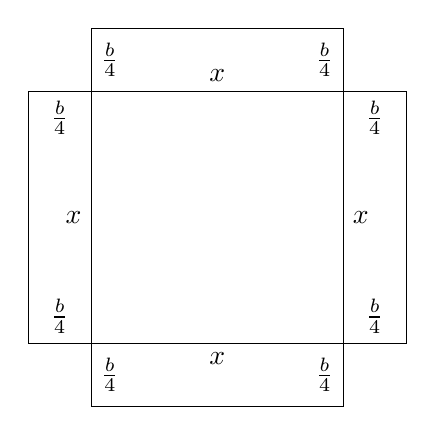
\begin{tikzpicture}[scale=.8]
\coordinate (A) at (0,0);
\coordinate (B) at (4,0);
\coordinate (C) at (4,4);
\coordinate (D) at (0,4);
\draw (A) -- node[below] {$x$} (B) -- node[right] {$x$} (C) -- node[above] {$x$} (D) -- node[left] {$x$} cycle;
\draw (A) -- node[right] {$\frac{b}{4}$} ++(0,-1) -- ++(4,0) -- node[left] {$\frac{b}{4}$} ++(0,1);
\draw (B) -- node[above] {$\frac{b}{4}$} ++(1,0) -- ++(0,4) -- node[below] {$\frac{b}{4}$} ++(-1,0);
\draw (C) -- node[left] {$\frac{b}{4}$} ++(0,1) -- ++(-4,0) -- node[right] {$\frac{b}{4}$} ++(0,-1);
\draw (D) -- node[below] {$\frac{b}{4}$} ++(-1,0) -- ++(0,-4) -- node[above] {$\frac{b}{4}$} ++(1,0);
\end{tikzpicture}
\caption{Das Gebiet ist $x^2+4(b/4)x=x^2+bx$}\label{f.khw-1}
\end{minipage}
\hfill
\begin{minipage}{.45\textwidth}
\begin{tikzpicture}[scale=.8]
\coordinate (A) at (0,0);
\coordinate (B) at (4,0);
\coordinate (C) at (4,4);
\coordinate (D) at (0,4);
\draw (A) -- node[below] {$x$} (B) -- node[right] {$x$} (C) -- node[above] {$x$} (D) -- node[left] {$x$} cycle;
\draw (A) -- node[right] {$\frac{b}{4}$} ++(0,-1) -- ++(4,0) -- node[left] {$\frac{b}{4}$} ++(0,1);
\draw (B) -- node[above] {$\frac{b}{4}$} ++(1,0) -- ++(0,4) -- node[below] {$\frac{b}{4}$} ++(-1,0);
\draw (C) -- node[left] {$\frac{b}{4}$} ++(0,1) -- ++(-4,0) -- node[right] {$\frac{b}{4}$} ++(0,-1);
\draw (D) -- node[below] {$\frac{b}{4}$} ++(-1,0) -- ++(0,-4) -- node[above] {$\frac{b}{4}$} ++(1,0);
\draw[thick,dashed] ($(A)+(0,-1)$) -- ++(-1,0) -- ++(0,1);
\draw[thick,dashed] ($(B)+(0,-1)$) -- ++(1,0) -- ++(0,1);
\draw[thick,dashed] ($(C)+(0,1)$) -- ++(1,0) -- ++(0,-1);
\draw[thick,dashed] ($(D)+(0,1)$) -- ++(-1,0) -- ++(0,-1);
\end{tikzpicture}
\caption{Das Gebiet ist $x^2+4(b/4)x+4(b/4)^2=x^2+bx+(b^2/4)$}\label{f.khw-2}
\end{minipage}
\end{figure}

Wir können das Diagramm in Abb.~\ref{f.khw-1} nicht konstruieren, weil wir nicht wissen, was $x$ ist, aber die Fläche des größeren Quadrats in Abb.~\ref{f.khw-2} ist:
\[
x^2+bx+\frac{b^2}{4}=c+\frac{b^2}{4}\,,
\]
was wir wissen, da uns die Koeffizienten $b,c$ gegeben sind. Durch die Konstruktion des Diagramms und das Löschen der kleinen Quadrate, deren Seiten $(b/4)$ sind - eine weitere bekannte Größe -, erhalten wir den Linienabschnitt der Länge $x$.

\begin{example}
Es sei $x^2+12x=64$. Dann sei $c+(b^2/4)=64+36=100$. Es ist leicht, ein Quadrat mit dem Flächeninhalt $100$ zu konstruieren, denn jede Seite hat die Länge $10$. Nun subtrahiert man $(b/4)+(b/4)=6$, die Seiten der kleineren Quadrate, und erhält $x=10-6=4$.
\end{example}

\section{Cardano's Konstruktion zur Lösung kubischer Gleichungen}\label{s.cardano}

Die Formel für die Wurzeln von kubischen Gleichungen wurde erstmals im 16. Jahrhundert von Gerolamo Cardano veröffentlicht. Wir werden die Formel hier nicht weiterentwickeln, aber es ist interessant, dass die zentrale Idee auf einer geometrischen Konstruktion beruht, die der von al-Khwarizmi ähnelt. Die Konstruktion lässt sich mit Hilfe der Algebra sehr einfach ermitteln. Durch Multiplikation:
\begin{align}\label{eq.car}
(a+b)^3=a^3+3a^2b+3ab^2+b^3=(a^3+b^3)+3ab(a+b)\,.
\end{align}
Geometrisch gehen wir von einem Würfel aus, dessen Seitenlänge $a+b$ beträgt, so dass sein Volumen $(a+b)^3$ ist. Der Würfel wird in fünf Teile zerlegt. Die ersten beiden sind Würfel mit den Seitenflächen $a$ und $b$ und den Volumina $a^3$ (blau) bzw. $b^3$ (rot) (Abb.~\ref{f.cardano1}).

Die anderen drei Teile sind Kästchen (der Fachbegriff lautet \emph{cuboid}), von denen jedes eine Seite der Länge $a+b$ hat, die mit einer Seite des Würfels zusammenfällt, eine Seite der Länge $a$ und eine Seite der Länge $b$, so dass das Volumen jedes der drei Kästchen $ab(a+b)$ beträgt. In Abb.~\ref{f.cardano2} befindet sich ein Kasten an der linken Seite des Würfels (blau), einer an der Rückseite des Würfels (rot) und einer an der Oberseite des Würfels (grün).
Kombiniert man die fünf Körper in Abb.~\ref{f.cardano1} und Abb.~\ref{f.cardano2}, erhält man Gl.~\ref{eq.car}.


\begin{figure}[htb]
\begin{center}
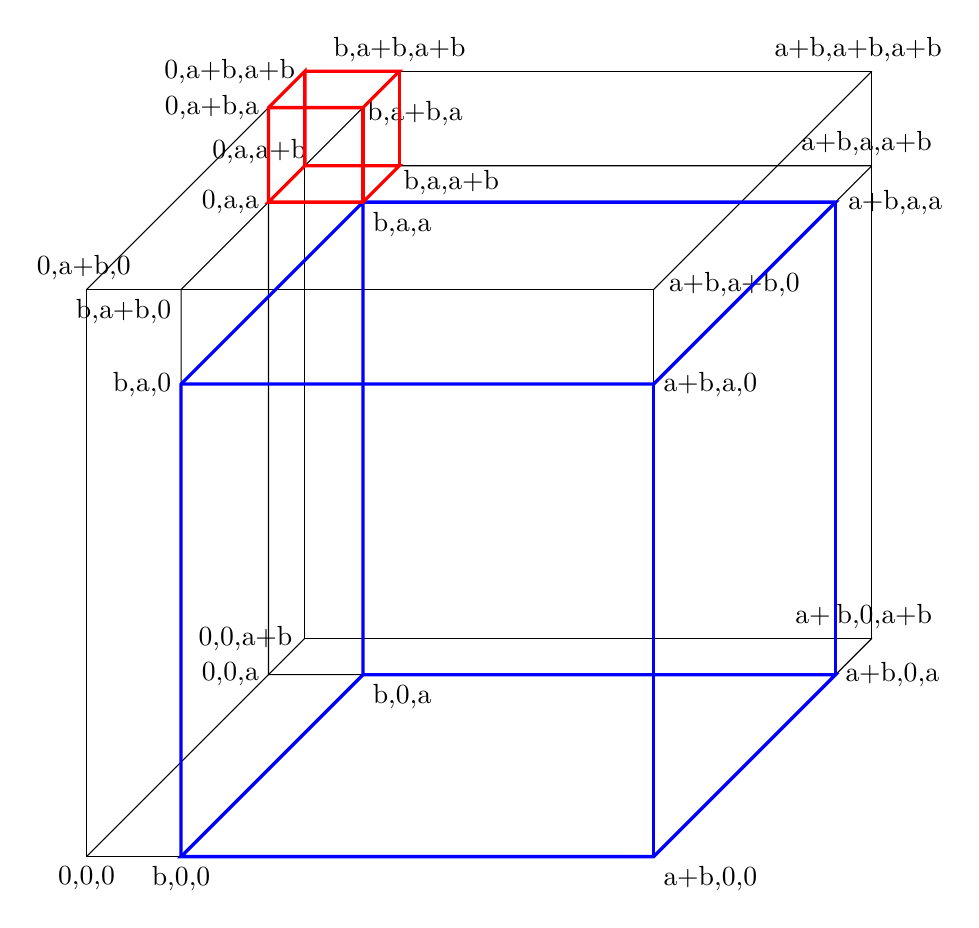
\begin{tikzpicture}[scale=1.2]

% Front face
\coordinate (A) at (0,0,0);
\node[below] at (A) {\sm{0,0,0}};
\coordinate (B) at (6,0,0);
\node[below right] at (B) {\sm{a+b,0,0}};
\coordinate (C) at (6,6,0);
\node[above right,xshift=2pt,yshift=-6pt] at (C)
  {\sm{a+b,a+b,0}};
\coordinate (D) at (0,6,0);
\node[above,xshift=-1pt] at (D) {\sm{0,a+b,0}};

% Front face
\coordinate (FF1) at (1,0,0);
\node[below] at (FF1) {\sm{b,0,0}};
\coordinate (FF2) at (1,5,0);
\node[left] at (FF2) {\sm{b,a,0}};
\coordinate (FF3) at (1,6,0);
\node[below left] at (FF3) {\sm{b,a+b,0}};
\coordinate (FF4) at (6,5,0);
\node[right] at (FF4) {\sm{a+b,a,0}};

% Back face
\coordinate (A1) at (0,0,-6);
\node[left,xshift=-1pt] at (A1) {\sm{0,0,a+b}};
\coordinate (B1) at (6,0,-6);
\node[above,xshift=-3pt] at (B1) {\sm{a+\:b,0,a+b}};
\coordinate (C1) at (6,6,-6);
\node[above,xshift=-5pt] at (C1) {\sm{a+b,a+b,a+b}};
\coordinate (D1) at (0,6,-6);
\node[left] at (D1) {\sm{0,a+b,a+b}};

% Back face
\coordinate (BF1) at (0,5,-6);
\node[above left,xshift=4pt,yshift=-3pt] at (BF1) 
  {\sm{0,a,a+b}};
\coordinate (BF2) at (1,5,-6);
\node[below right,xshift=-2pt,yshift=2pt] at (BF2)
  {\sm{b,a,a+b}};
\coordinate (BF3) at (1,6,-6);
\node[above] at (BF3) {\sm{b,a+b,a+b}};
\coordinate (BF4) at (6,5,-6);
\node[above,xshift=-2pt] at (BF4) {\sm{a+b,a,a+b}};

% Right face
\coordinate (RF1) at (6,5,-5);
\node[right,xshift=1pt] at (RF1) {\sm{a+b,a,a}};
\coordinate (RF2) at (6,0,-5);
\node[right] at (RF2) {\sm{a+b,0,a}};

% Bottom face
\coordinate (BT1) at (1,0,-5);
\node[below right] at (BT1) {\sm{b,0,a}};

% Left face
\coordinate (LF1) at (0,0,-5);
\node[left] at (LF1) {\sm{0,0,a}};
\coordinate (LF2) at (0,5,-5);
\node[left] at (LF2) {\sm{0,a,a}};
\coordinate (LF3) at (0,6,-5);
\node[left] at (LF3) {\sm{0,a+b,a}};

% Top face
\coordinate (TF1) at (1,6,-5);
\node[right,xshift=-2pt,yshift=-2pt] at (TF1) {\sm{b,a+b,a}};

% Internal point
\coordinate (I) at (1,5,-5);
\node[below right] at (I) {\sm{b,a,a}};


\draw (A) -- (B) -- (C) -- (D) -- cycle;
\draw (A1) -- (B1) -- (C1) -- (D1) -- cycle;
\draw (A) -- (A1);
\draw (B) -- (B1);
\draw (C) -- (C1);
\draw (D) -- (D1);

\draw (FF1) -- (FF2) -- (FF3) -- (BF3);
\draw (BF2) -- (FF2) -- (FF4) -- (BF4);
\draw (FF1) -- (BT1) -- (TF1);
\draw (BF3) -- (BF2);
\draw (TF1) -- (LF3);
\draw (LF3) -- (LF1) -- (RF2) -- (RF1) -- (LF2) -- 
      (BF1) -- (BF4);

\draw[very thick,blue] (FF1) -- (B) -- (RF2) -- (BT1) -- cycle; 
\draw[very thick,blue] (FF1) -- (FF2) -- (I) -- (BT1);
\draw[very thick,blue] (I) -- (RF1) -- (FF4) -- (FF2);
\draw[very thick,blue] (FF4) -- (B);
\draw[very thick,blue] (RF1) -- (RF2);

\draw[very thick,red] (I) -- (LF2) -- (BF1) -- (BF2) -- cycle;
\draw[very thick,red] (LF2) -- (LF3) -- (D1) -- (BF1);
\draw[very thick,red] (D1) -- (BF3) -- (TF1) -- (LF3);
\draw[very thick,red] (TF1) -- (I);
\draw[very thick,red] (BF3) -- (BF2);

\end{tikzpicture}
\end{center}
\caption{$(a^3+b^3)=(a^3+b^3)+\cdots$}\label{f.cardano1}
\end{figure}

%%%%%%%%%%%%%%%%%%%%%%%%%%%%%%%%%%%%%%%%%%%%%%%%%%%%%%%%%%%%%

\begin{figure}[htb]
\begin{center}
\begin{tikzpicture}[scale=1.2]

% Front face
\coordinate (A) at (0,0,0);
\node[below] at (A) {\sm{0,0,0}};
\coordinate (B) at (6,0,0);
\node[below right] at (B) {\sm{a+b,0,0}};
\coordinate (C) at (6,6,0);
\node[above right,xshift=2pt,yshift=-6pt] at (C)
  {\sm{a+b,a+b,0}};
\coordinate (D) at (0,6,0);
\node[above,xshift=-1pt] at (D) {\sm{0,a+b,0}};

% Front face
\coordinate (FF1) at (1,0,0);
\node[below] at (FF1) {\sm{b,0,0}};
\coordinate (FF2) at (1,5,0);
\node[left] at (FF2) {\sm{b,a,0}};
\coordinate (FF3) at (1,6,0);
\node[below left] at (FF3) {\sm{b,a+b,0}};
\coordinate (FF4) at (6,5,0);
\node[right] at (FF4) {\sm{a+b,a,0}};

% Back face
\coordinate (A1) at (0,0,-6);
\node[left,xshift=-1pt] at (A1) {\sm{0,0,a+b}};
\coordinate (B1) at (6,0,-6);
\node[above,xshift=-3pt] at (B1) {\sm{a+\:b,0,a+b}};
\coordinate (C1) at (6,6,-6);
\node[above,xshift=-5pt] at (C1) {\sm{a+b,a+b,a+b}};
\coordinate (D1) at (0,6,-6);
\node[left] at (D1) {\sm{0,a+b,a+b}};

% Back face
\coordinate (BF1) at (0,5,-6);
\node[above left,xshift=4pt,yshift=-3pt] at (BF1) 
  {\sm{0,a,a+b}};
\coordinate (BF2) at (1,5,-6);
\node[below right,xshift=-2pt,yshift=2pt] at (BF2)
  {\sm{b,a,a+b}};
\coordinate (BF3) at (1,6,-6);
\node[above] at (BF3) {\sm{b,a+b,a+b}};
\coordinate (BF4) at (6,5,-6);
\node[above,xshift=-2pt] at (BF4) {\sm{a+b,a,a+b}};

% Right face
\coordinate (RF1) at (6,5,-5);
\node[right,xshift=1pt] at (RF1) {\sm{a+b,a,a}};
\coordinate (RF2) at (6,0,-5);
\node[right] at (RF2) {\sm{a+b,0,a}};

% Bottom face
\coordinate (BT1) at (1,0,-5);
\node[below right] at (BT1) {\sm{b,0,a}};

% Left face
\coordinate (LF1) at (0,0,-5);
\node[left] at (LF1) {\sm{0,0,a}};
\coordinate (LF2) at (0,5,-5);
\node[left] at (LF2) {\sm{0,a,a}};
\coordinate (LF3) at (0,6,-5);
\node[left] at (LF3) {\sm{0,a+b,a}};

% Top face
\coordinate (TF1) at (1,6,-5);
\node[right,xshift=-2pt,yshift=-2pt] at (TF1) {\sm{b,a+b,a}};

% Internal point
\coordinate (I) at (1,5,-5);
\node[below right] at (I) {\sm{b,a,a}};


\draw (A) -- (B) -- (C) -- (D) -- cycle;
\draw (A1) -- (B1) -- (C1) -- (D1) -- cycle;
\draw (A) -- (A1);
\draw (B) -- (B1);
\draw (C) -- (C1);
\draw (D) -- (D1);

\draw (FF1) -- (FF2) -- (FF3) -- (BF3);
\draw (BF2) -- (FF2) -- (FF4) -- (BF4);
\draw (FF1) -- (BT1) -- (TF1);
\draw (BF3) -- (BF2);
\draw (TF1) -- (LF3);
\draw (LF3) -- (LF1) -- (RF2) -- (RF1) -- (LF2) -- 
      (BF1) -- (BF4);

\draw[very thick,blue] (A) -- (FF1) -- (FF3) -- (D) -- cycle;
\draw[very thick,blue] (FF1) -- (BT1) -- (TF1) -- (FF3);
\draw[very thick,blue] (TF1) -- (LF3) -- (D);
\draw[very thick,blue] (LF3) -- (LF1) -- (A);
\draw[very thick,blue] (LF1) -- (BT1);

\draw[very thick,red] (LF1) -- (RF2) -- (RF1) -- (LF2);
\draw[very thick,red] ($(LF2) + (2pt,0)$) -- ($(LF1) + (2pt,0)$);
\draw[very thick,red] (A1) -- (B1) -- (BF4) -- (BF1) -- cycle;
\draw[very thick,red] ($(LF2) + (2pt,0)$) -- ($(BF1) + (2pt,0)$);
\draw[very thick,red] (BF4) -- (RF1);
\draw[very thick,red] (B1) -- (RF2);
\draw[very thick,red] (A1) -- (LF1);

\draw[very thick,green] (FF2) -- (FF4) -- (C) -- (FF3);
\draw[very thick,green] 
  ($(FF2) + (2pt,0)$) -- ($(FF3) + (2pt,0)$);
\draw[very thick,green] 
  ($(FF4) + (0,2pt)$) -- ($(BF4) + (0,2pt)$);
\draw[very thick,green] (BF4) -- (C1) -- (BF3);
\draw[very thick,green] 
  ($(BF3) + (2pt,0)$) -- ($(FF3) + (2pt,0)$);
\draw[very thick,green] (C1) -- (C);
\draw[very thick,green] (BF3) -- (BF2) -- (FF2);
\draw[very thick,green] 
  ($(BF2) + (0,2pt)$) -- ($(BF4) + (0,2pt)$);


\end{tikzpicture}
\end{center}
\caption{$(a^3+b^3)=\cdots+3ab(a+b)$}\label{f.cardano2}
\end{figure}

\section{Sie ließen sich von imaginären Zahlen nicht einschüchtern}\label{s.imaginary}

Die Geschichte der Mathematik zeigt eine Reihe von Konzepten, die zunächst als bedeutungslos galten, aber schließlich verstanden und akzeptiert wurden und sich als nützlich erwiesen. Offensichtlich", da Zahlen Dinge zählen, ist $-1$, eine negative Zahl, bedeutungslos. Da Zahlen Verhältnisse von ganzen Zahlen (rationalen Zahlen) sind, ist $\sqrt{2}$, das sich leicht als irrational erweisen lässt, offensichtlich bedeutungslos. Offensichtlich ist $\sqrt{-1}$, die Quadratwurzel einer negativen Zahl, bedeutungslos, da es keine Zahl - weder eine ganze noch eine rationale oder reelle - gibt, deren Quadrat $-1$ ist.

Ein vollständiges Verständnis der Quadratwurzeln negativer Zahlen, die bis heute als imaginäre Zahlen bezeichnet werden, obwohl sie nicht weniger real sind als reelle Zahlen, wurde erst im neunzehnten Jahrhundert erreicht. Daher ist es erstaunlich, dass sich Geralamo Cardano und Rafael Bombelli bereits im 16. Jahrhundert nicht von dem Konzept einschüchtern ließen und die ersten kleinen Schritte zum Verständnis dieser Zahlen unternahmen.

Betrachten wir die quadratische Gleichung:
\begin{align}
x^2-10x+40=0\,.\label{eq.cardano-quadratic}
\end{align}
Nach der bekannten Formel (Gl.~\ref{eq.quadratic-roots}):
\[
r_1, r_2=\displaystyle\frac{10\pm\sqrt{100-160}}{2}=5\pm\sqrt{-15}\,.
\]
Nun, wir wissen nichts über die Quadratwurzeln negativer Zahlen und wir wissen nicht, was diese Werte sind, aber wie Cardano wissen wir durch Thm~\ref{eq.quadratic-roots}, dass:
\[
\begin{array}{lcl}
r_1+r_2&=&(5+\sqrt{-15})+(5-\sqrt{-15})=10=-b\\
r_1r_2&=&(5+\sqrt{-15})(5-\sqrt{-15})=25-5\sqrt{-15}+5\sqrt{-15}-(-15)=40=c\,.
\end{array}
\]
die mit den Koeffizienten der quadratischen Gleichung Gl.~\ref{eq.cardano-quadratic} übereinstimmen. Es ist ziemlich intuitiv, dass $\sqrt{-15}+(-\sqrt{-15})=0$, auch wenn wir nichts über $\sqrt{-15}$ wissen, und ebenso ist es ziemlich intuitiv, dass $\sqrt{-15}\cdot-(\sqrt{-15})=-(-15)=15$, auch wenn wir nicht wissen, was $\sqrt{-15}$ ist.

Betrachten wir nun die kubische Gleichung:
\begin{align}
x^3-15x-4=0\,.\label{eq.bombelli-cubic}
\end{align}
Es ist nicht schwer zu erkennen, dass $4$ eine Wurzel ist, aber wie kann man sie berechnen? Mit der Cardano-Formel erhält man die Wurzel:
\begin{align}
r=\sqrt[3]{2+11\sqrt{-1}}+\sqrt[3]{2-11\sqrt{-1}}\,,\label{eq.cube-root}
\end{align}
eine recht komplizierte Formel, die keinen offensichtlichen Bezug zu $4$ hat. 

Bombelli hat mutig die folgende Berechnung durchgeführt (siehe Gl.~\ref{eq.car}):
\begin{eqnarray*}
(2+\sqrt{-1})^3&=&
8+3\cdot 4\sqrt{-1}+3\cdot 2(-1)+(-1\sqrt{-1})=
2+11\sqrt{-1}\\
(2-\sqrt{-1})^3&=&
8-3\cdot 4\sqrt{-1}+3\cdot 2(-1)-(-1\sqrt{-1})=
2-11\sqrt{-1}\,,
\end{eqnarray*}
und durch Gl.~\ref{eq.cube-root}:
\begin{eqnarray*}
r&=&\sqrt[3]{2+11\sqrt{-1}} + \sqrt[3]{2-11\sqrt{-1}}\\
&=&\sqrt[3]{(2+\sqrt{-1})^3} + \sqrt[3]{(2-\sqrt{-1})^3}\\
&=&(2+\sqrt{-1}) + (2-\sqrt{-1})=4\,.
\end{eqnarray*}

%%%%%%%%%%%%%%%%%%%%%%%%%%%%%%%%%%%%%%%%%%%%%%%%%%%%%%%%

\section{Die Lillsche Methode und der Carlyle'sche Kreis}\label{s.lill-quadratic}

Die Lill-Methode kann zur Lösung quadratischer Gleichungen verwendet werden. Fußnote{Dieser Abschnitt setzt voraus, dass Sie die Lill-Methode in Kap.~\ref{c.origami-cube}.}\index{Lill-Methode!quadratische Gleichungen} gelesen haben. Als Beispiel dient die Gleichung ~\ref{eq.quadratic-lill}, die die Wurzeln einer quadratischen Gleichung durch Faktorisierung angibt:
\[
x^2+bx+c=x^2-4x+3= (x-1)(x-3)\,.
\]
Die Anwendung der Lill'schen Methode führt zu den in Abb.~\ref{f.lill-quadratic} dargestellten Pfaden.

\begin{figure}[bt]
\begin{center}
\begin{tikzpicture}[scale=1.1]
% Draw help lines and axes
\draw[step=10mm,white!50!black] (-4,-5) grid (2,1);
\draw[thick] (-4,0) -- (2,0);
\draw[thick] (0,-5) -- (0,1);
\foreach \x in {-3,...,2}
  \node at (\x-.2,.2) {\sm{\x}};
\foreach \y in {-4,...,-1}
  \node at (-.2,\y-.3) {\sm{\y}};

 Draw first path
\coordinate (A) at (0,0);
\coordinate (B) at (1,0);
\coordinate (C) at (1,-4);
\coordinate (D) at (-2,-4);
\draw[very thick] (A) --
  node[above] {$1$} (B);
\draw[very thick,name path=bc] (B) -- 
  node[right,xshift=-1pt,yshift=6pt] {$b=-4$} (C);
\draw[very thick,name path=cd] (C) --
  node[below left,xshift=3pt] {$c=3$}(D);

% Draw first segment of second path
\path[name path=a2] (A) -- +(-45:1.414);
\path [name intersections = {of = a2 and bc, by = {A2}}];
\node[above right] at (A2) {$P_1$};
\draw[very thick,dashed] (A) -- (A2);
\draw ($(A) + (14pt,0)$)
  arc [start angle=0, end angle = -45, radius=14pt];
\node[below right,xshift=40pt,yshift=-2pt] at (A) {$-45^\circ$};
\draw[->] ($(A)+(33pt,-6pt)$) -- +(-18pt,0);
\draw[rotate=135] (A2) rectangle +(5pt,5pt);

% Draw second segment of second path
\path[name path=b2] (A2) -- +(-135:5);
\path [name intersections = {of = b2 and cd, by = {B2}}];
\draw[very thick,dashed] (A2) -- (B2);

% Draw first segment of second path
\path[name path=a3] (A) -- +(-71.57:4);
\path [name intersections = {of = a3 and bc, by = {A3}}];
\node[above right] at (A3) {$P_2$};
\draw[very thick,dashed] (A) -- (A3);
\draw ($(A) + (20pt,0)$)
  arc [start angle=0, end angle = -71.57, radius=20pt];
\node[below right,xshift=40pt,yshift=-10pt] at (A) {$-71.57^\circ$};
\draw[->] ($(A)+(35pt,-13pt)$) -- +(-18pt,0);
\draw[rotate=108.43] (A3) rectangle +(5pt,5pt);

% Draw second segment of second path
\path[name path=b3] (A3) -- +(198.43:5);
\path [name intersections = {of = b3 and cd, by = {B3}}];
\draw[very thick,dashed] (A3) -- (B3);

\end{tikzpicture}
\end{center}
\caption{Lills Methode auf $x^2-4x+3$}\label{f.lill-quadratic}
\end{figure}
Prüfen Sie, ob die Winkel korrekt sind:
\[
-\tan (-45^\circ) = -1,\quad -\tan (-71.57^\circ) \approx -3\,.
\]
Für quadratische Gleichungen können wir die Punkte $P_1,P_2$ als Schnittpunkte der Linie, die den Koeffizienten $b$ darstellt, und des Kreises finden, dessen Durchmesser die Verbindungslinie zwischen dem Anfangs- und dem Endpunkt der Wege ist (Abb.~\ref{f.lill-circle}). Damit ein Punkt auf der Geraden $b$ eine Wurzel ist, muss die Spiegelung der Geraden $90^\circ$ sein, und daher wird der eingeschriebene Winkel durch einen Durchmesser begrenzt.

\begin{figure}[t]
\begin{center}
\begin{tikzpicture}[scale=1]
% Draw help lines and axes
\draw[step=10mm,white!50!black] (-4,-5) grid (2,1);
\draw[thick] (-4,0) -- (2,0);
\draw[thick] (0,-5) -- (0,1);
\foreach \x in {-3,...,2}
  \node at (\x-.2,.2) {\sm{\x}};
\foreach \y in {-4,...,-1}
  \node at (-.2,\y-.3) {\sm{\y}};

 Draw first path
\coordinate (A) at (0,0);
\coordinate (B) at (1,0);
\coordinate (C) at (1,-4);
\coordinate (D) at (-2,-4);
\draw[very thick] (A) --
  node[above] {$1$} (B);
\draw[very thick,name path=bc] (B) -- 
  node[right,xshift=-2pt,yshift=6pt] {$b=-4$} (C);
\draw[very thick,name path=cd] (C) --
  node[below left,xshift=-1pt,yshift=-5pt] {$c=3$}(D);

% Draw first segment of second path
\path[name path=a2] (A) -- +(-45:1.414);
\path [name intersections = {of = a2 and bc, by = {A2}}];
\node[above right] at (A2) {$P_1$};
\draw[dashed] (A) -- (A2);
\draw ($(A) + (14pt,0)$)
  arc [start angle=0, end angle = -45, radius=14pt];
\node[below right,xshift=40pt,yshift=-2pt] at (A) {$-45^\circ$};
\draw[->] ($(A)+(33pt,-6pt)$) -- +(-18pt,0);
\draw[rotate=135] (A2) rectangle +(5pt,5pt);

% Draw second segment of second path
\path[name path=b2] (A2) -- +(-135:5);
\path [name intersections = {of = b2 and cd, by = {B2}}];
\draw[dashed] (A2) -- (B2);

% Draw first segment of second path
\path[name path=a3] (A) -- +(-71.57:4);
\path [name intersections = {of = a3 and bc, by = {A3}}];
\node[above right] at (A3) {$P_2$};
\draw[dashed] (A) -- (A3);
\draw ($(A) + (20pt,0)$)
  arc [start angle=0, end angle = -71.57, radius=20pt];
\node[below right,xshift=40pt,yshift=-10pt] at (A) {$-71.57^\circ$};
\draw[->] ($(A)+(35pt,-13pt)$) -- +(-18pt,0);
\draw[rotate=108.43] (A3) rectangle +(5pt,5pt);

% Draw second segment of second path
\path[name path=b3] (A3) -- +(198.43:5);
\path [name intersections = {of = b3 and cd, by = {B3}}];
\draw[dashed] (A3) -- (B3);

\coordinate (O) at (-1,-2);
\vertex{O};
\node[draw,circle through=(A)] at (O) {};
\draw[very thick,dotted] (A) -- (D);

\end{tikzpicture}
\end{center}
\caption{Konstruktion eines Kreises zur Ermittlung der Wurzeln}\label{f.lill-circle}
\end{figure}

Dies kann auch rechnerisch überprüft werden. Der Mittelpunkt des Kreises ist der Mittelpunkt des Durchmessers $(-1,-2)$. Die Länge des Durchmessers ist:
\[
\sqrt{(-2)^2+(-4)^2}=\sqrt{20}\,,
\]
Das Quadrat der Länge des Radius ist also $\left(\sqrt{20/2}\right)^2=5$. Wir brauchen den Schnittpunkt dieses Kreises mit der Linie $x=1$:
\begin{eqnarray*}
(x-(-1))^2+(y-(-2))^2&=&r^2\\
(x^2+2x+1)+(y^2+4y+4)&=&5\\
y^2+4y+3&=&0\\
y&=&-1,\;-3\,.
\end{eqnarray*}
Eine ähnliche Methode zum Lösen quadratischer Gleichungen ist der Carlyle-Kreis, der der Lill-Methode vorausgeht. Bei einer quadratischen Gleichung $x^2-bx+c$ (beachten Sie das Minuszeichen des linearen Terms) konstruieren Sie die Punkte $(0,1)$ und $(b,c)$. Konstruieren Sie einen Kreis, dessen Durchmesser die Verbindungslinie zwischen den beiden Punkten ist (Abb.~\ref{f.carlyle-circle}). Seine Schnittpunkte (falls vorhanden) mit der $x$-Achse sind die Wurzeln der Gleichung.

Im allgemeinen Fall ist der Mittelpunkt des Kreises $(b/2,(c-(-1))/2)$ und die Länge des Durchmessers $\sqrt{b^2+(c-1)^2}$, so dass die Gleichung des Kreises lautet:
\[
\left(x-\frac{b}{2}\right)^2+\left(y-\frac{c+1}{2}\right)^2=
\frac{b^2+(c-1)^2}{4}\,.
\]
Wenn man im Beispiel $b=4,c=3$ und $y=0$ einsetzt, sieht man, dass $x=1$ und $x=3$ die Wurzeln der quadratischen Gleichung sind.

\begin{figure}[t]
\begin{center}
\begin{tikzpicture}[scale=1]
% Draw help lines and axes
\draw[step=10mm,white!50!black] (-1,-1) grid (5,5);
\draw[thick] (-1,0) -- (5,0);
\draw[thick] (0,-1) -- (0,5);
\foreach \x in {0,...,5}
  \node at (\x-.2,.2) {\sm{\x}};
\foreach \y in {1,...,4}
  \node at (-.1,\y+.2) {\sm{\y}};

\coordinate (A) at (0,1);
\node[below left] at (A) {$(0,1)$};
\coordinate (B) at (4,3);
\node[above right] at (B) {$(4,3)$};
\vertex{A};
\vertex{B};

\coordinate (O) at (2,2);
\vertex{O};
\node[draw,circle through=(B)] at (O) {};
\draw[very thick,dotted] (A) -- (B);

\coordinate (X1) at (1,0);
\node[below left] at (X1) {$(1,0)$};
\coordinate (X2) at (3,0);
\node[below right] at (X2) {$(3,0)$};
\vertex{X1};
\vertex{X2};

\end{tikzpicture}
\end{center}
\caption{Carlyle-Kreis für $x^2-4x+3$}\label{f.carlyle-circle}
\end{figure}

\section{Numerische Berechnung der Wurzeln}\label{s.numerical}
\index{Quadratic equation!numerical computation of the roots}

Die Schüler lernen die symbolische Berechnung von Wurzeln, Ableitungen und so weiter. Heutzutage werden die meisten Berechnungen von Computern durchgeführt, so dass symbolische Berechnungen weniger wichtig sind. Die \emph{numerische Analyse} ist der Zweig der Mathematik und Informatik, der genaue und effiziente Berechnungsmethoden entwickelt. Die größte Herausforderung besteht darin, mit der Endlichkeit der im Speicher des Computers gespeicherten Werte umzugehen. Die Berechnung:
\[0.12\times 0.14=0.0168\]
ist leicht zu machen, aber:
\[
0.123456789\times 0.123456789
\]
braucht achtzehn Ziffern, um genau dargestellt zu werden, und das kann nicht in einem Speicherwort geschehen, das sechzehn Ziffern speichert. Dieser Fehler wird als \emph{Abrundungsfehler} bezeichnet.

Ein noch schwerwiegenderes Problem tritt auf, wenn eine Fließkommaarithmetik durchgeführt wird. Das ist klar:
\[(0,12\times 10^{-10})\times (0,14\times 10^{-8})\]
würde nicht durch Ausschreiben aller Nullstellen berechnet werden. Stattdessen werden die Mantissen multipliziert und die Exponenten addiert, um $0,0168\times 10^{-18}$ zu erhalten, das auf $0,168\times 10^{-19}$ normiert wird, so dass die höchstwertige Ziffer nach dem Dezimalpunkt erscheint, was angesichts der festen Größe der Mantisse eine maximale Genauigkeit gewährleistet. Wenn der maximal darstellbare Exponent $-16$ beträgt, kann das Ergebnis gar nicht gespeichert werden. Dieser Fehler wird als \emph{Gleitkomma-Unterlauf} bezeichnet.\index{Gleitkomma-Unterlauf}

Die Formel für die Suche nach den Wurzeln der quadratischen Gleichung $x^2+bx+c$ lautet:
\begin{align}
r_1, r_2 = \frac{-b\pm\sqrt{b^2-4c}}{2}\,.\label{eq.quadratic-numerical}
\end{align}
Überlegen Sie, was passiert, wenn $b=1000$ und $c=4$. Die Wurzeln sind:
\[
r_1, r_2 = \frac{-1000\pm\sqrt{1000000-16}}{2}\,.
\]
Je nach Rechengenauigkeit ist es möglich, dass eine der Wurzeln so nahe an Null liegt, dass der gespeicherte Wert Null ist. Die Auswertung der quadratischen Gleichung ergibt das überraschende Ergebnis $0^2+b\cdot 0 +4= 4= 0$.

Können wir es besser machen? Mit Gleichung ~\ref{eq.viete-quad}:
\[
r_1+r_2 = -b\,,\quad\quad r_1r_2=c\,.
\]
Wenn $r_2$ viel kleiner ist als $r_1$, also $r_2\ll r_1$, dann ist $r_1\approx -b$ und $r_2=c/b$. Die von einem Computerprogramm berechnete Tabelle~\ref{t.quadratic} vergleicht die Werte der mit diesen Formeln berechneten Wurzeln mit den Werten, die sich aus der traditionellen Formel Eq.~\ref{eq.quadratic-numerical} ergeben. Der Wert von $c$ ist auf $4$ festgelegt und die Wurzeln für steigende Werte von $b$ werden gezeigt.

Zunächst sind die wahren Werte, die mit der traditionellen Formel für $r_2$ berechnet werden, genauer ($r_2-r_{2v}$ ist negativ), aber ab $b=100000$ ist die Berechnung auf der Grundlage von Eq.~\ref{eq.viete-quad} genauer. Das sind die Überraschungen der numerischen Analyse.

\begin{table}[bht]
\caption[Zwei Berechnungen der Wurzeln einer quadratischen Gleichung]{Zwei Berechnungen der Wurzeln einer quadratischen Gleichung. $r_1,r_2$ sind die durch Gl.~\ref{eq.quadratic-numerical} berechneten Wurzeln. $r_{1v},r_{2v}$ sind die mit Gl.~\ref{eq.viete-quad} berechneten Wurzeln. Die Fehler sind $r_{i}-r_{iv}$. Die Werte werden auf vier Dezimalstellen abgeschnitten.
Fließkommazahlen werden mit $-4e-5$ anstelle von $4\times 10^{-5}$ geschrieben, weil Computerprogramme normalerweise als lineare Folgen von Zeichen geschrieben werden.} \label{t.quadratic}
\[
\begin{scriptsize}
\begin{array}{r@{\hspace{2.5mm}}r@{\hspace{2.5mm}}r@{\hspace{2.5mm}}r@{\hspace{2.5mm}}r@{\hspace{2.5mm}}r@{\hspace{2.5mm}}r}
\hline
\noalign{\smallskip}
b & r_1 & r_{1v} & \mathrm{Error}_1 & r_2 & r_{2v} & \mathrm{Error}_2\\
\noalign{\smallskip}\hline\noalign{\smallskip}
100  &  -99.9599  &  -100  &  0.0400  &  -0.04001\  &  -0.04  &  -1.6012e\!-\!05\\
1000  &  -999.9959  &  -1000  &  0.0040  &  -0.0040  &  -0.004  &  -1.6000e\!-\!08\\
10000  &  -9999.9996  &  -10000  &  0.0004  &  -0.0004  &  -0.0004  &  -1.6270e\!-\!11\\
100000  &  -99999.9999  &  -100000  &  3.9999e\!-\!5  &  -3.9999e\!-\!5  &  -4e\!-\!5  &  1.0104e\!-\!12\\
1000000  &  -999999.9999  &  -1000000  &  4.0000e\!-\!6  &  -3.9999e\!-\!6  &  -4e\!-\!6  &  2.7749e\!-\!11\\
10000000  &  -10000000.0  &  -10000000  &  3.9860e\!-\!7  &  -3.9953e\!-\!7  &  -4e\!-\!7  &  4.6261e\!-\!10\\
 \noalign{\smallskip}
 \hline
\end{array}
\end{scriptsize}
\]
\end{table}

\subsection*{Was ist die Überraschung?}

Der Ansatz von Poh-Shen Loh bietet eine neue Sichtweise auf die Beziehung zwischen den Koeffizienten und den Wurzeln, die man nicht sieht, wenn man sich nur die traditionelle Formel merkt. Überraschend ist, dass diese Beziehung in Gauß' algebraischem Beweis für die Konstruierbarkeit eines regelmäßigen Heptadecks (Kap.~\ref{c.heptadecagon}) von grundlegender Bedeutung ist.

Angesichts der modernen Dominanz algebraischer Methoden in der Geometrie ist es wichtig, sich daran zu erinnern, dass das Gegenteil einst galt. Wie die Konstruktionen von Al-Khwarizmi und Cardano zeigen, wurden geometrische Methoden verwendet, um Ergebnisse in der Algebra zu erhalten. Lill und Carlyle entwickelten beide geometrische Methoden zur Lösung quadratischer Gleichungen. Die Überlegungen zur numerischen Berechnung auf Computern werden die Schüler überraschen, die noch keine Erfahrung damit haben.

\subsection*{Quellen}
Die Methode von Poh-Shen Loh stammt aus \cite{loh1,loh2}. Al-Khwarizmis Konstruktion stammt aus \cite[Chapter~1]{jorg} und \cite{mastin}. Cardanos Konstruktion ist in \cite[Kap.~1]{jorg} zu finden. Für die bunte Geschichte der Entwicklung der Cardano-Formel siehe \cite{wiki:cardano}. Die frühen Versuche, mit imaginären Zahlen zu rechnen, finden sich in \cite[Chapter~2]{jorg}. Lills Methode und Carlyles Kreis sind in \cite{wiki:quad} zusammen mit einer Diskussion der numerischen Berechnung der Wurzeln zu finden.
